\documentclass[12pt,a4paper]{article}
\usepackage[a4paper]{geometry}
\usepackage{array}
\usepackage{hhline}
\usepackage{graphics}
\usepackage{csvsimple}
\usepackage[russian,english]{babel}
\usepackage[utf8]{inputenc}
\usepackage[T2A]{fontenc} 
\usepackage{ulem}
\usepackage{cmap}
\usepackage{makecell}
\usepackage{ifpdf}
\setlength\extrarowheight{2pt}
\setlength{\parindent}{0cm}
\newcommand{\phylentry}[6] {\\\hline\makecell{
#1\medskip\\
\hhline{|-|}
\\#2\\#3\medskip\\
\hhline{|-|}\\
{#6}}
&\makecell{#4}&\makecell{#5}}
%Syntax: \phylentry{Who}{When}{Where}{Phylosophy}{NotPhylosophy}{ETC} // currently ETC is not used
\hoffset -1.6cm 
\textwidth  16.5cm 
\textheight 24cm 
%\topmargin -1cm 
\parskip 8pt 
\setlength{\unitlength}{1cm}
\sloppy
\addto\captionsenglish{
\renewcommand{\contentsname}{{\bf CO}ntents}
\renewcommand{\refname}{Bibliography}
\renewcommand{\figurename}{Figure}
\renewcommand{\tablename}{Table}
\renewcommand{\abstractname}{Abstract}
\renewcommand{\partname}{Section}
\renewcommand{\bottomfraction}{0.5}
\renewcommand{\floatpagefraction}{0.4}
\renewcommand{\textfloatsep}{0.5cm}
\renewcommand{\intextsep}{0.6cm}
\renewcommand{\floatsep}{0.3cm}
}

\renewcommand\theadalign{cb}
\renewcommand\theadfont{\bfseries}
\renewcommand\theadgape{\Gape[4pt]}
\renewcommand\cellgape{\Gape[4pt]}
%<pics>
\newcommand{\materialist}[0]{\includegraphics{dummy-achievement.png}}%</pics>
\begin{document}
%..................................................................
\begin{titlepage}
\par 
\vspace*{-2cm}
\begin{center}
{\sf \Large
\vspace*{1.5cm}
{\Huge Семенов, 9-й семестр, 2017}\\
{ Философия, эпизод 2:}\\
{ Больше конспектов \sout{Богу} Абсолютному духу конспектов}}\\

\vspace*{2cm}
\scalebox{1.2}{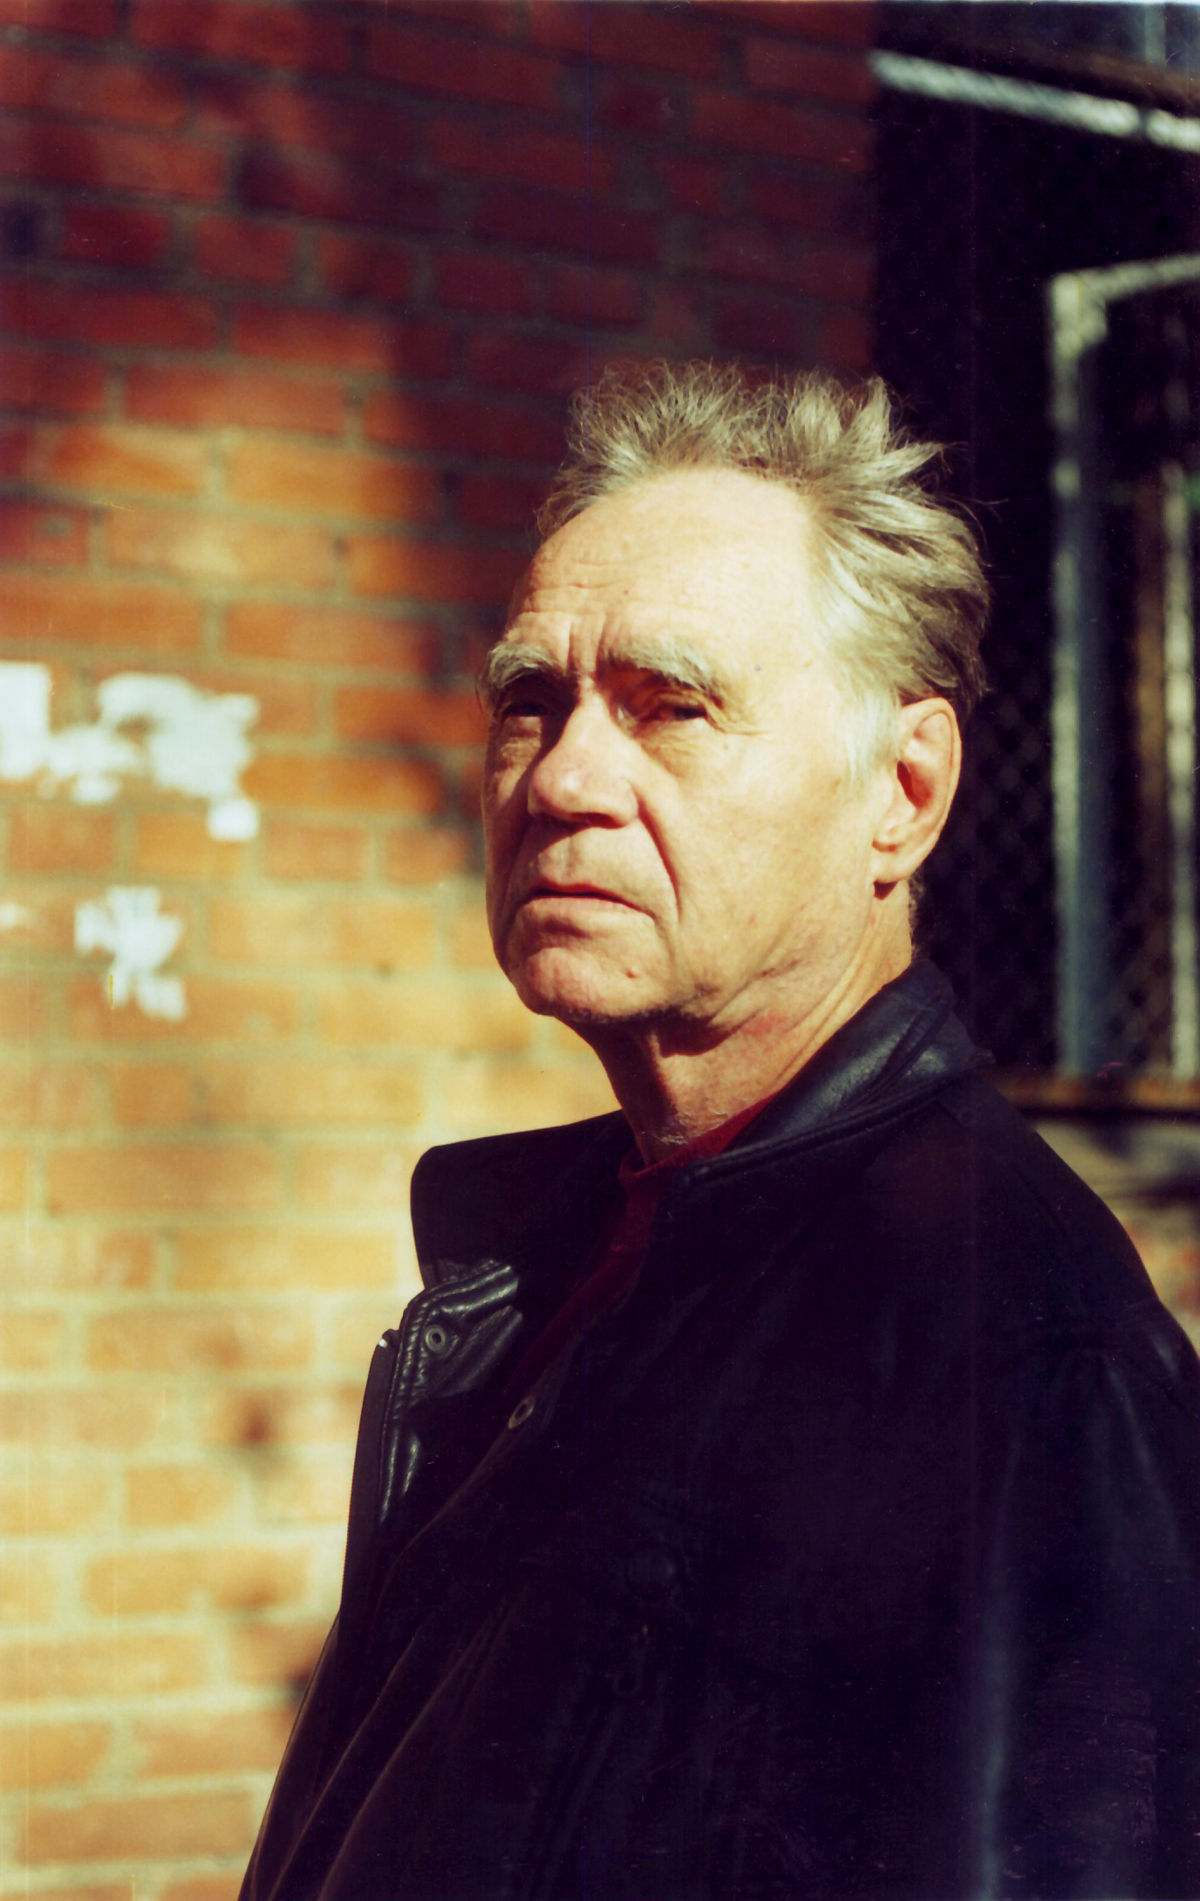
\includegraphics{thegod.jpg}} \\
{\small }
\begin{flushright}
\sl\small
by Nyaxx-11k aka KingKO
\end{flushright}
\end{center}
\end{titlepage}
%..................................................................
\topmargin -1cm 
\hoffset -0.7in 
\textwidth 6.0in 
\textheight 9.0in 
\normalsize 
\pagenumbering{arabic}
%----------------
\tableofcontents
\pagebreak
%----------------

\section{Научная революция XVII века}
Наука окончательно сформировалась в 17 в. \textit{Вообще, знание было всегда, но раньше оно было бессистемным и бездоказательным. В Древнем Египте, например, умели решать квадратные уравнения, но рецепт был получен методом тыка. Первое доказательство появилось только в 6 в. д.н.э. (привет, Фалес Милетский). Тогда, правда, наука смешивалась с натурфилософией аки нейтрино. С вытекающими отсюда переходами одного в другое. Окончательно же труЪ-наука сформировалась в 17 в.}
Ну и пробежимся по ученым того времени (спискота):

\underline{Леонардо да Винчи (1452-1519)}. Художник, изобретатель. Человек у него лишь первый из зверей, а душа не бессмертна. Один из первых \textbf{эмпириков} - ценил опыт, но и чистый эмпиризм без анализа отвергал. Развивал математику.

\underline{Николай Коперник (1473-1543)}. В книге "Об обращении небесных сфер" ввел математически обоснованную гелиоцентрическую систему. Утверждал, что это лишь способ уточнить расчеты (правда, его модель была далеко не идеальна). Говорил, что это гипотетически, боялся публиковаться. Еще бы - Церкви это ой как не понравилось. Правда, Церковь тогда была занята реформацией, а потом работа разошлась, а Коперник в тот же год благоразумно умер, и все: поздняк метаться, Земля - не центр мироздания, Бог не может жить на небесной тверди по причине отсутствия оной. Пришлось закинуть Бога за орбиту Сатурна (то, что есть еще Уран и Нептун, никто не догадывался).

\underline{Джордано Бруно (1548-1600)}. Философ, естествоиспытатель. В работах жег не по-детски. Мир бесконечен, звезды - те же солнца, с планетами и разумной жизнью. Инопланетян что, тоже Христос создал? Вот и получается, что Бога нет. Да, в Средневековье была популярна концепция двух истин - разума и откровения. Так вот, нет двух истин - есть только истина разума, а религия - бред собачий.  Правда, мировая душа у него все-таки была, но это нечто глобальное и пассивное. У церкви с такого пригорело, однако в 1600 году на Площади Цветов во Флоренции она взяла реванш. Особый цинизм ситуации заключался в том, что костер считался гуманной казнью, так как не приводил к пролитию крови. \textit{Однако, эпопея с горящими задницами продолжается. Так, недавно поставили Джордано на этой самой Площади Цветов памятник - дескать, мученик науки, сгорел на работе, можно сказать (\textit{Вечный огонь поставьте}). Так вот, верующие раскукарекались. А узнай Джордано, что в 21 веке в одной стране поп кандидатскую по теологии защитил - сгорел бы и без дров.}

\underline{Галилео Галилей (1564-1642)}. Астроном, создатель первого телескопа (правда, подзорная труба была уже до него). Изучил Луну. Открыл спутники Юпитера (4 самых крупных). Еще и механик - опроверг положение Аристотеля о разной скорости падения тел. Изучал динамику пушечного ядра - даже в баллистики приглашали. Ну и маятник. Написал "Диалог о двух системах мира" (Птолемей vs Коперник - защищает Коперника). Написал на итальянском, а не на латыни. Слетелись инквизиторы и заставили публично отречься. Галилей отрекся (есть легенда, что в конце он произнес "И все-таки она вертится". Пруфов нет).  

\underline{Иоганн Кеплер (1571-1646)}. Опять астроном, открыл три закона обращения планет (\textit{вспомним общефиз, 1-й семестр?})

\underline{Уильям Гильберт (1540-1603)}. \textit{Не путать с Давидом Гильбертом - тот из 20-го века.} Наука и до Англии добралась. Изучал магнит, открыл джва его полюса, понял, что у Земли тоже есть магнитное поле. Еще изучал электростатику, открыл, что не только янтарь электризуется.

\underline{Уильям Горвей (1578-1657)}. Открыл кровообращение. Основоположник физиологии и эмбриологии.

\underline{Эванжелиста Торричелли (1608-1646)}. Открыл атмосферное давление и изобрел ртутный барометр. Создал гидродинамику.

\underline{Отто фон Герике (1602-1686)}. Изобрел воздушный насос, поставил опыт со сферой из двух половинок, в которой был вакуум, и которую не могли разнять две упряжки. 

\underline{Роберт Бойль (1627-1691)}. Открыл закон имени себя-Мариотта. Создал научную химию.

\underline{Эдм Мариотт (1620-1684)}. Открыл закон имени Бойля-себя. Создал французскую академию наук.

\underline{Христиан Гюйгенс (1629-1691)}. Открыл кольца Сатурна, создал маятниковые и пружинно-балансирные часы. Моряки сказали спасибо, ибо без них долготу корабля фиг определишь. Создал теорию маятника и волновую теорию света.

\underline{Антон ван Левенгук (1632-1723)}. Изобрел микроскоп. Открыл бактерии, и запилил микробиологию. \textit{А однажды плюнул под микроскоп. Посмотрев на зоопарк полости рта, стал чистить зубы еще до того, как это стало мейнстримом.}

\underline{Роберт Гук (1635-1705)}. Закон имени себя.

\underline{Исаак Ньютон (1642-1716)}. 3 закона имени себя + закон всемирного тяготения + матан, независимо от Лейбница. Сделал механику точной наукой. Топил за корпускулярную теорию света - \textit{создатель квантмеха (нет)}
 
На этом спискота все. Итого 12 ученых. А если в общем - ученые стали ставить эксперименты (систематические), юзать приборы - всякие теле-микро-скопы, баро-термометры, часы. Появились обсерватории. В Англии Карл II запилил первую академию наук - т.н. "Королевское общество" (1662). Потом тренд подхватили Франция, Пруссия, а там и в Россию завезли. Ученые стали делать доклады, а сборники этих докладов стали первой научной прессой. Потом, когда ученых стало побольше, уже и нормальная периодика пошла. Появилось и научное мышление. Чудеса наука не рассматривала. Да, гнать на церковь по-прежнему было накладно, но это уже шаг вперед . Появилась концепция \textbf{детерминизма} - учения о всеобщей причинности и предопределенности событий. Потом и теорвер появился. Он с детерминизмом прекрасно уживался - все случайности проистекают из нашего недостаточного знания, а на самом деле все предопрелелено. Тут нужно упомянуть Лапласа с его демоном. Если демон знает коориднаты и скорости всех тел, а также имеет бесконечную разрядность и производительность, он сможет просчитать все события в нашем мире. Такой вот \textbf{механистический детерминизм}. \textit{Правда, квантовая механика похоронила абсолютный детерминизм, но в пропатченных вариантах он жив}.
%Smth else?

\section{Западноевропейская классическая философия XVII - первой половины XIX вв. Эмпиризм и рационализм.}
Итак, окончательно сформировалась наука. И тем самым у философов появилась пища для ума. Откуда берется научное знание? Как мыслить так, чтобы полученные теории действительно работали? \textit{Тут нужно сказать, что есть два вида знания - \textbf{житейское} и \textbf{научное}. Первое - бессистемное и бездоказательное, полученное в ходе повседневной человеческой деятельности. Второе же и системное, и обосновывается. Например, счет на пальцах у древних людей - это житейское знание. А аксиоматика Пеано - научное}. Надо сказать, еще Бэкон (который Роджер) выделял три источника знания - авторитет, ум и опыт. То, что авторитет может ошибаться - и так понятно. А с умом и опытом сложнее. И тут возникли два направления - \textbf{эмпиризм} и \textbf{рационализм}.

Эмпиристы утверждают, что единственный источник знания - опыт (Р. Бэкон, к слову, тоже придерживался этой мысли). \textbf{Априорного}, т.е. полученного без опыта знания у них нет - только  \textbf{апостериорное}. Да, самое главное: а что есть \textbf{опыт}? Ну, опыт бывает житейский и научный. С ними все примерно так же, как и со знанием. Житейский получается в ходе человеческой практики - хочешь, чтобы что-то заработало - делай так-то, а так-то, наоборот, не делай. Научный - продуманный, системный, знание, полученное в ходе него, фиксируется в суждениях, т.е. становится \textbf{фактом}. Нельзя сказать, что все эмпирики отвергают разум: многим он нужен для обработки экспериментальных данных в теории. Т.е. сначала эмпирический уровень знания, а потом и теоретический. Есть же и \textbf{сенсуалисты} - у них в разуме нет ничего, чего не было бы в чувствах (\textit{ага, многие из вас видели отдельные атомы?}).

Рационалисты, напротив, говорили, что априорное знание есть, и более того, оно даже круче апостериорного: опыт может раз сработать, два сработать, а на третий раз слажать, а вот что доказано умом - то работает всегда.

А где же истина? А она, как всегда, где-то рядом. Действительно, мир дан нам только в наших чувствах - правы сенсуалисты. Но разум в состоянии раскрывать закономерности, находить причинно-следственные связи и создавать реально работающие (разумеется, с определенной точностью и в определенных границах) теории - правы рационалисты. Так что, все эти направления - это, как правило, раздувание одной стороны истины в ущерб другим.

\section{Философия Френсиса Бэкона}
\underline{Френсис Бэкон (1561 - 1626)}. Англичанин. Не был старшим сыном, а потому остался без земли в наследство. Пришлось кончить Оксфорд и работать адвокатом. Был близок ко Двору. В 1603 оборвалась жизнь Елизаветы I, а вместе с ней и династия. Взошел на престол Якоб I (по Шотландии уже Якоб VI; если быть точнее, James VI). При нем Бэкон стал лордом-хранителем печати, а потом (16!8) и лордом-канцлером. Правда, потом карьера его пошла под откос: в 1621-и парламент, решив насолить королю, привлек Бэкона за взяточничество и злоупотребление властью. Коррумпированный лорд получил 40к штрафа, запрет на работу в сфере политики и камеру в Тауэре "до освобождения". Король, правда, отменил первые два наказания, потом и ко двору допустили, но осадочек остался. В итоге, отсидел Бэкон только два дня (\textit{привет, Васильева}). Карл I, сев на трон, и вовсе хотел восстановить Бэкона в должности, но тот отакзался.

Бэкон писал книги. Нам нужен его опус 1620-го года \textbf{"Новый органон"} (\textit{В пику "старому" Органону - набору работ Аристотеля по логике.}). Наука у него - высшая форма знания о природе.
Не нравилось Бэкону, что как-то на практике теория не шибко юзается.  Он выдвинул три тезиса:
\begin{enumerate}
\item Объект научного познания - природа.
\item Задача науки - познавать природу.
\item Цель - подчинить природу человеку.
\end{enumerate}
Ну и конечно, для познания нужен метод. Его Бэкон и хотел запилить. Итак, начнем с его четырех препятствий для ученого ака \textbf{четырех идолов}:
\begin{enumerate}
\item Идол рода: в мышление вносят искажения природа человека и тело человека . 
\item Идол пещеры: знание ограничено. Всегда кажется, что все уже открыли.
\item Идол площади/(\textit{у анкапов сейчас подгорит})рынка - существует множество точек зрения, в том числе популярных и неверных. Надо бы  от них отказатья, а общественное мнение не дает.
\item Идол театра: древние мыслители и авторитеты. Они могут ошибаться.
\end{enumerate}

Источник знания - чувства. Таки да, \textbf{эмпирист}, но не радикальный: знание - не просто набор фактов. Ученых делил на три категории:
\begin{enumerate}
\item Муравьи. Просто таскают факты в муравейник.
\item Пауки. Тянут из себя теории без опоры на факты.
\item Пчелы. А вот эти годные: сначала собирают факты-нектар, а потом фигачат из них мед-теорию. \textit{И летают.}
\end{enumerate}

Аристотель в Органоне изучал только дедукцию. В Новом же Органоне разбирается индукция и построенная на ней логика. Для этого есть методы \textbf{сходства}/\textbf{различия}/\textbf{выявления причин}. Ну и до кучи еще термины: \textbf{анализ} - расчленение на части; \textbf{синтез} - соединение в целое. Семенов приводил пример: анализ - тяжелое, пластичное, желтое, синтез - золото. \textbf{Форма} у Бэкона - законы и сущности явлений. У него 19 форм движения - механистическим редукционизмом не страдал.

\section{Философия Рене Декарта}
\underline{Рене Декарт(1596 - 1650)}. Он же Картезиус на латыни. Человек и система координат. Учился в Иезуитском колледже, потом дропнул и пошел работать. Был из дворянского рода, но младшим сыном. Как наемник пошел в армию, причем сразу в офицеры (дворянин же). Опять дропнул и уехал в Голландию философствовать. В Голландии тогда прошла буржуазная революция, вероисповедание свободное, Республика семи провинций. Запилил книжку "Размышление о методе \textit{<там полное длинное заглавие, но и так сойдет>}". В этой книжке - 4 правила для исследователя:
\begin{enumerate}
\item За основу берутся очевидно истинные положения.
\item Дальше они \textbf{анализируются} - расчленяются на составные части.
\item А потом \textbf{синтезируются} воедино, от простого к сложному.
\item Всегда проверяется, не упущено ли что-либо важное.
\item ?????????
\item PROFIT
\end{enumerate}
Источники знания у него:
\begin{enumerate}
\item Самое главное - априорные идеи (\textit{ну вы чувствуете, какой \textbf{рационалист}?}). Они и так очевидны.
\item Интуиция.
\item Дедукция.
\end{enumerate}
Да, априорные идеи. Во-первых, я мыслю, а следовательно существую. Т.е существует мыслящая субстанция.
Во-вторых, существует Б-г - это врожденная идея. В-третьих, есть вещи - о них говорит Б-г (\textit{блин, ну Декарт}). А значит есть протяженная субстанция. Мир у него существует в пространстве и времени, но они - такая же материя. Это \textbf{реляционная} концепция, в пику \textbf{субстанциональной}. Да, Декарт \textbf{дуалист} - у него и мир первичен, и сознание. Да не совсем - их сначала создал Б-г, который все-таки скорее сознание. Правда, потом Б-г на мир забил (\textbf{деизм-с}), и они как бы оба первичны, но слив идеализму засчитан. Планеты и звезды у него появиись из облака мельчайших частиц (за подробностями уже к Канту с Лапласом). \textbf{Механист}, и как сказано ранее, \textbf{деист}: Бог создал законы, а дальше все само собралось. Животные у него - просто куски материального мира, управляемые рефлексами (уже разделял врожденные и приобретенные). А вот человек - единство души и тела.

\section{Философия Томаса Гоббса}
\underline{Томас Гоббс (1588 - 1679)}. Родился в семье служащего. Тоже кончил Оксфорд, дальше пошел в домашние учителя для богатых людей (Это весьма частая завязка биографий). Путешествовал по Европе.  Изучил "Начала" Евклида. Проникшись строгостью математики, захотел того же от других наук. Написал труд "О гражданине" - книгу об обществе. Во Франции сблизился с английской королевской семьей. \textit{Стопчто?! С английской королевской семьей во Франции?! Ну, там было так... Захотел Карл I запилить новый налог в 1641-м. Собрал парламент. А блэд  пэрлэмэнт потребовал наказать коррупционеров. Лорду-канцлеру пришлось отрубить голову. Не успокоились. Началась революция, гражданская война. Короля поймали, он бежал, потом снова поймали, судили, и в итоге он, как и лорд-канцлер, попрощался с головой. А вот семья таки успешно завела трактор.
% Кстати, Гоббс критиковал применение силы в работе "О гражданине", а так как Кромвель и Ко именно что применением силы и занимались,  пришлось Гоббу валить -- PROOFS NEEDED
} Так вот, Гоббс с ними сблизился, потом поссорился. Накатал "Левиафана" - там топил за сильное государство. Там же вводит концепцию общественного договора. Кромвелю, который к тому моменту сосредоточил власть в своих руках, понравилось. А потом Кромвель умер. Король вернулся, то теперь его повязали по рукам и ногам конституцией. 

Итак, это была биография Гоббса. А теперь его взгляды. Вообще, они изложены в трех его работах: "О теле", "О человеке", "О гражданине". \textbf{Материалист}. Значение науки для него огромно. Она строится на фактах, но их необходимо переработать в теорию. А для этого, опять-таки, нужен метод. \textit{Ах да, теологию высмеивал. Так ей и надо.} В его терминологии чувствуется тяга к матану. Так, он все "складывал" и "вычитал". Ввел понятие \textbf{метки} - вещи, заставляющей вспомнить о чем-либо, и \textbf{знака} - вещи, метки, юзаемой в общении (\textit{слова, например}). Крайний \textbf{номиналист}, хотя и  сбивался к умеренному. Мир у него - гигантская совокупность тел - телесная субстанция (\textit{чувствуется материализм}) - она вечна. Декарта критиковал - мышление - свойство высокоорганизованной субстанции, а не сама субстанция. Мир существует во времени и пространстве. Есть и движение, но тут Гоббс - \textbf{механистический редукционист}. Как почти неизбежное следствие этого, \textbf{абсолютный детерминист}, отрицал теорию \textbf{двух истин}, чудеса, \sout{заговор жидомасонов с иллюминатами и плоскую Землю}. Отрицал даже свойства типа цвета, вкуса и запаха - типа это порождение сознания (\textit{Демокрит, привет}). Мир имеет двоякое бытие - сам по себе и в сознании. В сознании он отражается. 

А теперь, как двигать науку. Тут все почти то же самое: анализ, синтез и дедукция. Он заимствует идеи рационализма- геометрия, например, у него дает общее знание, ибо не опирается на опыт. Науки он делил на \textbf{индуктивные} (опирающиеся на эмпирические факты, например, физика) и \textbf{дедуктивные} (например, геометрия или наука об обществе).

Люди у него сначала жили без норм и понятия о собственности. Каждый сталкивался с каждым - "Война всех против всех". Во избежание этого, были запилены государство и собственность. Формы государства три - республика, аристократия и абсолютная монархия (Гоббс именно ее и уважает). Атеист, но религия у него нужда, дабы \sout{быдло} народ не бунтовал.

\section{Философия Баруха Спинозы}
\underline{Барух (Бенедикт) Спиноза (1632 - 1677)}. Родился в Республике семи провинций (нынешняя Голландия). Родился в Амстердаме, в гетто - таки евrей. Учился в еврейской школе, изучал Ветхий завет. Думали, способный малый, богослов будет - ан нет, малый действительно оказался способный - положил на синагогу свой обрезанный и ушел в Латинскую школу. Ему предлагали хотя бы делать вид, что иудаист - отказался. Устроили сначала малое, а потом и великое отлучение (1656) - выперли из общины. Пошел к ван Эйдену, но евреи добились его изгнания из города как безбожника. Голландия, конечно, была веротерпимой, но вовсе не атеистотерпимой. Так и осел Спиноза в деревне. Шлифовал линзы и философствовал. В 1673 курфюрст Фальце пригласил в Гейдельбергский университет. Зарплата - во! Единственное - просьба поосторожнее высказывать мнение. Но Спиноза сломал стереотипы о евреях и атеизм на шекели не променял. Французы предложили одну из работ посвятить королю. Отказался - "Я свои работы посвящаю только истине!"

Сначала был \textbf{дуалист}. Потом - \textbf{монист}. Субстанция у него  - это Б-г (\textbf{пантеист}). Субстанция вечна, бесконечна в пространстве и времени, неделима и не состоит из частей, а еще она мыслит. Природу делит на \textbf{производящую} (собственно, Б-г) и творимую. Проявления субстанции носят название \textbf{модусов}. Это - вещи, они не вечны, движутся (\textit{Но субстанция неподвижна, аки у Парменида с Зеноном}). \textbf{Абсолютный детерминист} - есть всеобщая предопределенность. Но и свобода есть - это осознанное и добровольное подчинение необходимости.

Выделял четыре формы познания:
\begin{enumerate}
\item Знание понаслышке
\item Бессистемный опыт
\item Рассуждение
\item Интуиция - рр-раз, и допер. Интуиция не обманывает. Но и в мистику Спиноза не скатывается. Просто способность человека, которую он не осознает. 
\end{enumerate}
Таки \textbf{рационалист}. Религия возникает от невежества и страха перед природой, и должна быть побеждена просвещением. Наука опирается на факты. История в том числе, и к источникам же нужно относиться критически - когда создан, кем, откуда это кто-то узнал о событии. В принципе, Лоренцо Валла об этом уже говорил. Спиноза так покритиковал Библию. В частности, показал, что Пятикнижие Моисеево ака Тора написана точно не Моисеем. Причина проста: там есть описание смерти Моисея. А зомби вроде как в Библии отсутствуют (Лазарь не в счет, тем более что абилка на воскрешение только у Иисуса была).

\section{Философия Готфрида Лейбница}
\underline{Готтфрид Вильгельм Лейбниц (1646 - 1716)}. Родился в Лейпциге. Отец - профессор морали. Говорят, корни у Лейбница славянские (\textit{мамкиному националисту на заметку}). Работал в области науки и философии. Запилил счетную машину. Германия тогда еще не была буржуазной страной. Буржуазия была осторожной и шла на компромиссы. И философия Лейбница тоже. Хотел он науку с религией помирить. \textbf{Мех. редукционизм} не уважал. А вообще философия у него интересная. Он, как и Декарт, маргинал - не материалист и не идеалист (\textit{ну, как сказать не идеалист...}). Он \textbf{плюралист} - первично дофига всего. Его учение - \textbf{монадология}. Монада - субстанция; каждая сама по себе. Их бесчисленное множество. Они существуют вне времени и пространства, замкнуты на себя и не связаны друг с другом. Они неуничножимы, а, нет, есть высшая монада, которая может создавать и уничтожать остальные. Кто она? Б-г. Короче, \textbf{объективный идеализм} так и зияет через дыры в теории. Монады движутся и действуют. Без связи друг с другом - Б-г их откалибровал так, что достиг гармонии. Монады делятся на три сорта:

\begin{enumerate}
\item Голые. Неразвытые, без восприятия.
\item Души - уже есть восприятие ака \textbf{перцепция} (как животные).
\item Духи - у них и сознание ака \textbf{апперцепция} есть.
\end{enumerate}
Материя же - сложная субстанция из простых субстанций, т.е. монад. Материй у него два сорта. Первый - протяженная масса.
Второй - активная материя - находится в движении. В механицизм Лейбниц, как и было сказано ранее, не впадал. У него и появление качеств, и развитие - это формы движения.  Всякий покой только относителен. Есть и принцип сохранения силы - она не появляется и не исчезает, а только переходит из одного состояния в другое. В теории познания Лейбниц ставит во главу угла мышление - \textbf{рационалист}. Истин две (\textit{не путать со схоластикой!}) - истина разума, и случайная истина как результат эксперимента. А еще Лейбниц считал, что живет в наилучшем из возможных миров. И оправдывал Б-га (\textbf{теодецея}) - "Бог создал добро, а его нет без зла".


\section{Философия Джона Локка}
\underline{Джон Локк (1632 - 1704)}. Кончил Оксфорд. Отец участвовал в революции на стороне Парламента, был там капитаном. После Оксфорда Локк пошел преподавать, потом познакомился с лордом Эшли (ака графом Шефтсбери), оппозиционером. Стал его врачом. Когда лорд стал лорд-канцлером, Локк стал его секретарем, а когда началось преследование, свалил в Голландию. Вернулся только после т.н. "Славной революции", когда очередного короля (на этот раз Якова II) низложили. Славная - значит бескровная. 

В 1690 г. пишет "Опыт о человеческом разуме". \textbf{Эмпирист} - все  знание апостериорно, а человек рождается \textbf{tabula rasa} (лат. "с чистого листа"). Опыт у его двух сортов: \textbf{внешний} (предмет подествовал на органы чувств) и \textbf{внутренний}, ака опыт \textbf{рефлексии} - наблюдение разума за самим собой. \textit{Вообще, назвать опытом рефлексии мышление - значит маскировать рационалистические мысли.} От опыта появляются простые чувственные и рефлексивные идеи, которые уже превращаются мозгом в более сложные. Качества у него тоже двух видов - первичные (объем, вес и т.д.) и вторичные (цвет, вкус, звук и т.д.). Про них будет далее. Субстанция у него есть \textbf{телесная} и \textbf{мыслящая}. Сущность вещей у него непознаваема. Есть три формы познания - \textbf{интуиция} (очевидное) (\textit{Локка так и тянет в рационализм}), \textbf{демонстративное} познание (доказуемое) и \textbf{опытное/сенситивное} (ограничное). А еще он \textbf{деист}.

\section{Учение Джона Локка о первичных и вторичных качествах}
Качества у Локка двух видов - \textbf{первичные} (объем, вес и т.д.) и \textbf{вторичные} (цвет, вкус, звук и т.д.). Первые объективны и неотделимы от тел, вторые субъективны и в том виде, в котором человек их воспринимает, в телах не существуют.
% 
\section{Философия Джорджа Беркли}
\underline{Джордж Беркли (1685 - 1753)}. Окончил Тринити-колледж. Священник. Стал домашним священником одного дипломата. Потом и епископом стал. 

Решил, что материализм - фундамент атеизма, а посему, чтобы разрушить атеизм, надо развенчать материализм. \textit{Семенов против смешивания религии с идеализмом, кстати. Идеализм  все же научная теория (пусть даже Семенов считает ее неверной), а религия бездоказательна и включает в себя культ. Не поклонялись же философы Абсолютному духу.} Так вот, для пропаганды ХГМ Беркли выкатил прямо-таки антипод материализма - \textbf{субъективный идеализм}. Согласно нему, сознание не просто первично, а мир существует исключительно в моем сознании \textit{(Так и говорим - "в моем сознании". Не "в сознании Беркли")}. До кучи \textbf{крайний номиналист} - нет общего, и материи нет, ибо она - общее (\textit{еще бы она была - это сугубо безбожный материалистический термин, обозначающий объективное бытие}). Все состоит из чувств - ведь мир только в сознании. Быть - значит быть воспринимаемым. Вот и до \textbf{солипсизма} докатился. Манямир в сознании Беркли трещал по швам. Сначала, ему пришлось ввести мыслящих духов - иначе бы предметы пропадали, когда Беркли отворачивался от них и/или спал. Мыслящие духи, конечно воспринимали предметы, препятствуя их исчезновению, но исключительность моего сознания${}^\mathtt{TM}$ оказалась подорвана. Дальше, каждый безбожник-материалист, да и вообще каждый философ, еще не дофилософствовавшийся до психбольницы, не пытался наесться воображаемыми, скажем, яблоками. Но в Берклимире-то восприятие/представление и есть сам предмет! Пытавшись покукарекаться с тем, что представление какое-то бледное по сравнению с восприятием, Беркли в конце концов ввел-таки Бога, который должен был отделять одно от другого. \textit{Казалось бы, наличие Б-га доказано и материализм-атеизм побежден. Вин? А вот и нет, фейл. Дело в том, что такой Б-г - самый настоящий Абсолютный д-х. Вот и развился субъективный идеализм в свою противоположность - в объективный. А что, неплохая иллюстрация диалектики.} А еще Беркли писал книги. 1710 - "Трактат о принципах человеческого знания",  1713 - "Три диалога между Гиласом и Филонусом".

\section{Философия Давида Юма. Обоснование им феноменализма (агностицизма).}
\underline{Давид Юм (1711 - 1776)}. Шотландец, сын дворянина. Написал историю Англии (8 томов!) и историю религии. На интересует его "Трактат о человеческой природе". В двух частях. В первой исследовал познание, в второй - эмоции. в 40-м году дописал третью часть - учение о морали. в 48-м было запилено второе издание первой части - "Исследование человеческого познания". 

\textbf{Эмпирик} - единственный источник знания - опыт. Тут он заодно с Локком - есть \textbf{перцепция} и \textbf{рефлексия}. О рефлексии почти ничего не писал. Чувственный опыт делится на \textbf{представления} ака \textbf{идеи} - они бледные и тусклые, и на \textbf{впечатления/восприятия}, которые делятся на \textbf{простые} - отдельные чувства, и сложные - (восприятие целиком отдельного предмета). На вход подается чувственный материал, а дальше он обрабатывается - ищется:
\begin{enumerate}
\item Сходство.
\item Смежность (близость в пространстве).
\item Причинность.
\end{enumerate}
И знание тоже двух типов - частные и недоказуемые \textbf{факты}, и всеобщее и доказуемое знание, получаемое развертыванием идей (как математика).

Юм создал \textbf{агностицизм} - учение, в котором утверждается неразрешимость основоного вопроса философии. Объяснял он это так: вещь познана - значит она вошла в наше сознание. Следовательно, то, что в сознание не вошло (например, мир - если мы его знаем, то он в сознании)  -то непознаваемо. Это не значит, что ничто не познаваемо - содержание своего сознания мы знаем. На основной вопрос Юм дает три гипотетических ответа:
\begin{enumerate}
\item Да, есть вещи вне сознания
\item Нет, есть только наши представления
\item Нет, Б-г вкладывает мир в наши ощущения
\end{enumerate}
С точки зрения формальной логики не подкопаешься. \textit{Но Юма можно опровергнуть созданием теории, то есть с помощью разумного мышления. Однако, отпочковавшиеся от агностиков \textbf{позитивисты}, которые сейчас доминируют, такие доказательства не признают (а иногда и разум).}

А еще Юм был безбожником. Правда, для народа религия, по ему мнению нужна, а вот интеллектуальной элите - ни к чему.  

\section{Основные идеи века Просвещения}
А тем временем наступил 18 век ака век Просвещения. Установился Культ Разума (имеется в виду разум человечества). Даже Гимн Разуму запилили. Идея прогресса (т.е. того, что человечество таки развивается) окончательно восторжествовала.
Разум же захотел свободы, равенства (перед законом) и братства. Во Франции назревала революция (и даже началась под конец века). 

\section{Возникновение первых научных периодизаций мировой истории и концепции прогресса (человеческого общества Адам Фергюсон, Адам Смит, Жак Тюрго, Жан Кондорсе).}
Итак, наконец все поняли, что человечество развивается. Историю надо было периодизировать (\textit{нет, Иоахим Флорский не считается}).

\underline{Адам Фергюссон (1723 - 1816)} - запилил периодизацию истории в "Очерке истории гражданского общества" (1761). Народы делятся на "отесанные" - цивилизованные и "неотесанные" - диких людей и варваров. "Дикие" живут охотой и собирательством, иногда и земледелием. Короче, у них первобытный коммунизм. Цивилизованные - тоже все понятно. Государство. Варвары -  промежуточное звено между дикими и цивилизованным. Народы развиваются и проходят периоды один за другим.
\textit{Такие термины были и раньше. Открыли Америку, индейцев назвали дикими, себя - цивилизованными, а варвары - промежуточное звено}.

Следующими отметились француз \underline{Жак Тюрго (1727 - 1781)} и англичанин \underline{Адам Смит (1723 - 1790)} (тот самый, который экономист и написал книгу "Исследование о причинах и природе богатства народов). Выделяли уже четыре стадии:
\begin{enumerate}
\item Охота + Собирательство 
\item Приручение животных - скотоводство
\item Земледелие
\item Тогрово-промышленная стадия
\end{enumerate}

\underline{Жан-Антуан Кондорсе (1743 - 1793)} же написал "Эскиз исторической картины прогресса человеческого разума". За него считают родоначальником теории прогресса. Топил за выравнивание прав и дальнейшее совершенствование. А во Франции была революция. Осудил якобинцев, был объявлен врагом народа, пытался сбежать, умер в тюрьме еще до выяснения личности (\textit{один фиг гильотина светила}). 

\section{Жан-Жак Руссо, Морелли, Габриэль де Мабли}
% % % % % % % % % % % % % % % % % %
\section{Географический детерминизм. Ш. Монтескье.}
Географический детерминизм - концепция исторического развития, согласно которой главный фактор, определяющий развитие народов - география и среда обитания.

\underline{Шарль Монтескье (1689 - 1755)} - создатель концепции географического детерминизма. Написал книгу "О духе законов". Объяснял законы в таком духе: вот есть Северная Африка, там жарко, работать не хочется - нужно принудить - получили деспотизм; в Европе попрохладнее, так и так впахивают - режим полиберальнее. В Азии степи и деспотизм. Ну и почва. Если скудные - то демократия, если богатые - их хотят заграбастать и аристократия. \textit{А если есть нефть, то демократию приносят из-за океана}.  

\section{Демографический детерминизм.  К.А. Гельвеций и А. Барнав.}
Немного другая концепция - демографический детерминизм.  Там все определяется плотностью и размерами населения. Его представители - \underline{Клод-Адриен Гельвеций (1715 - 1780)} и \underline{Антуан Барнав (1761 - 1793)}. Последний запилил "Введение во Французскую революцию". Правда, демография не единственный фактор, но главный.

\section{Вольтер}
Автор проболел, покидайте ему конспектов.
% % % % % % % % % % % % % % % % % % % %
\section{Жан Мелье}
Автор проболел, покидайте ему конспектов.
% % % % % % % % % % % % % % % % % % %
\section{Борьба французских материалистов XVIII в. против идеализма и религии}
Автор проболел, покидайте ему конспектов.
% % % % % % % % % % % % % % % % % % % % % % %
\section{Учение французских материалистов XVIII в. о природе. Их механицизм и абсолютный детерминизм}
Автор проболел, покидайте ему конспектов.
% % % % % % % % % % % % % % % % % % % % % % % % %
\section{Теория познании французских материалистов}
Автор проболел, покидайте ему конспектов.
% % % % % % % % % % % % % % % % % % % % % % % %
\section{Учение французских материалистов XVIII в.  об обществе и истории}
Автор проболел, покидайте ему конспектов. Но кусочек Семенов рассказал. Были они почти последовательные материалисты, но с обществом лажали. Есть \textbf{Общественное мнение} - система значимых взглядом. Оно определяет деля людей, творящих общественную среду. Итого мысль первична, мир вторичен - вот и идеализм. Пытались вырваться, но безуспешно - человек не всегда по разуму, а иногда и по страстям. Откуда страсти? Природа человека? Не всегда. Интересы людей? А они откуда? Общественное мнение. Короче, этот вопрос пришлось оставить до появления \textbf{марксизма}. А в истории был \textbf{волюнтаризм} - историю двигают великие люди. Короче, тут ребята слились. Надо сказать, что \textbf{волюнтаризм} встречается до сих пор. \textbf{Неолибералы} \textit{(англ. \textbf{neoconservators}, почувствуй силу перевода!)}, например, в него ударяются только так. А, и абсолютный детерминизм оборачивается индетерминизмом. То есть, если все взаимосвязано, то мы ничего не можем предсказать, ибо все причины учесть не в состоянии. \textit{Эффект бабочки и динамический хаос в механических системах - это оно самое. }

\section{Иммануил Кант.  Жизнь и развитие его философской мысли.}
\underline{Иммануил Кант (1724 - 1804)}. Родился в Кенигсберге. Четвертый ребенок из девяти. Батя устроил в гимназию, затем в университет (1740-1747). Правда, диссертацию Кант не защитил (по тем временам это как диплом). Стал преподом для богатых детей. В 55-м диссертацию таки защитил. Стал приват-доцентом. Подрабатывал помощником библиотекаря в королевской библиотеке. В 70-м наконец дали профессора. Ознакомился с работами Руссо - зашли на ура. Запилил на пару с Лапласом теорию возникновения Солнечной системы из газопылевого облака (как Декарт, но уже с наукой). Еще выдвинул гипотезу, что Вселенная состоит из галактик (работа называлась "Естественная история неба"). В его творчестве выделяют \textbf{докритический} и \textbf{критический} периоды (принято делить по 70 году). Критический - от его работ: "Критика чистого разума" (1781), "Критика практического разума" (1788), и "Критика способности суждения" (1790). В 1793 запилил "Религию в пределах только разума". Получилось богохульно, король попросил больше такого креатива не выдавать. Кант пообещал не писать до тех пор, пока король жив. Еще у Канта есть про мораль и категорический императив, но в вопросах этого нет.

\section{Учение Иммануила Канта о ноуменах (вещах в себе) и феноменах (вещах для нас)}
В "Критике чистого разума" Кант решил выяснить границы человеческого познания. Знание есть \textbf{априорное} и \textbf{апостериорное} из опыта. Только априорное всеобщее - а это математика, теоретическое естествознание и метафизика. Причем первые две точно дают априорное знание, а вот метафизика - ХЗ. А дальше пошло познание:
\begin{enumerate}
\item Есть \textbf{ноумены} ака \textbf{вещи в себе}. Да, у Канта есть объективный мир. Нет, обмазаться идеализмом это ему не помешало.
\item Ноумены воздействуют на наши органы чувств, и мы воспринимаем \textbf{феномены} ака \textbf{явления} ака \textbf{вещи для нас} (последний термин ввели уже потом). Сходства с вещами в себе нет. Совсем. Абсолютно.
\end{enumerate} 
Итого наши чувства дают нам хаос, и их нужно упорядочить. Для этого есть две формы чувственного созерцания - время и пространство. Мышление у Канта делится на две ступени - рассудок и разум.

\section{Априоризм Иммануила Канта}
Итак, апостериорное знание не может быть всеобщим - оно же опытное, а там вещи в себе. А вот априорное всеобщее. Но его могут дать лишь математика, теоретическое естествознание и, может быть, метафизика. Априорное знание в данном случае - не врожденное. Формы чувственного созерцания - время и пространство - априорны. И они феноменальны - в мире вещей-в-себе их нет. Дальше Кант выкатывает $4\times3=12$ категорий рассудка (\textit{хотя де-факто их 17}): 

\begin{tabular}{|c|c|c|c|}
\hline
\textbf{Количество}& \textbf{Качество}& \textbf{Онтошение}& \textbf{Модальность}\\
\hline
Единство&Реальность&Субстанция и принадлежность&Возможность и невозможность\\
\hline
Множество&Отрицание&Причина и следствие&Существование \\&&&и несуществование\\
\hline
Цельность&Ограничение&Взаимодействие&Случайность и необходимость\\
\hline
\end{tabular}
Эти категории были  для человечества в целом, но для нас уже априорны. Эти ощущения синтезируются -\textbf{категориальный синтез}.
Все категории берутся из разума. 
Знание - результат синтеза чувств и мышления. Мышление строит мир-сам-по-себе из чувственного материала. Да, Кант допер, что познание - не пассивное отражение, а творение. \textit{Но увлекся}. Пытался доказать объективность мира ("трансцендентальное единство апперцепции" - Кант любит извращенные формулировки). Задача разума - добиться истины. Эта задача неразрешима, но если очень хочется, но нельзя, то можно. У разума возникают три трансцендентальные идеи:
\begin{enumerate}
\item Психологическая - идея о душе как о единстве сознаний
\item Космологическая - идея о мире и космосе, как о единстве явлений.
\item Теологическая - идея о Б-ге, как о первопричине
\end{enumerate}
из них вырастают рациональные психология, космология и теология. Они, естественно, не работают, ибо мир, душа и Б-г - вещи в себе (\textit{а последнего вообще нет}). Развенчал одно за другим доказательства бытия Бога.

\section{Иммануил Кант о синтезе чувственности и рассудка}
Знания даются чувственным и категориальным синтезом.

\section{Открытия Иммануила Канта. Рациональное зерно, содержащееся в его гносеологической концепции.}
Кант, конечно, хорош, но он увлекся. Познание - не пассивное отражение, а творение. Кант решил - или - или. ТО, что это последовательное отражение и творение одновременно, не понял.  В антиномиях он открыл единство противоположностей, но не понял этого и не сумел в диалектику.

\section{Иммануил Канта о разуме. Антиномии разума.}
Итак, разум пытается построить картину мира, но закономерно терпит фейл. Кант формулирует 4 антиномии
\begin{enumerate}
\item Конечен ли мир в пространстве и времени? Ни да, ни нет.
\item Мир единый или составной? Ни да, ни нет.
\item Есть ли свобода? Или абсолютный детерминизм? В мире-для-нас детерминизм, в мире вещей-в-себе - свобода. 
\item Есть ли создатель? И да, и нет.
\end{enumerate}

\section{Жизнь и философия Иоганна Готлиба Фихте}
\underline{Иоганн Готлиб Фихте (1764 - 1814)}. Родился в деревне Рамена в Саксонии. Отец - ремесленник и землевладелец. Пятый ребенок в семье. Бегал на проповеди к священнику, оправдывая свое второе имя (\textit{нем. Gottlieb - боголюб}). А еще на проповеди ходил барон фон Мильтиц. Однажды он опоздал. Тут появился Фихте и пересказал проповедь (в 9 лет). Барон проникся мощью гения, и сначала отправил в сельскую школу, а потом в интернат для дворян. Пока Фихте учился, барон умер. Наследникам же проповедей никто не читал, и после интерната Фихте уже никто не спонсировал. Поступил в Йенский университет (\textit{конечно же на богословие}), потом перебрался в Лейпциг, но денег не было, и держаться Фихте уже не мог. Как и многие другие, пошел в домашние преподы. Проникся Кантом, в 1791-м наконец добрался до его лекции. В 1792 написал "Критику всякого откровения". Анонимно. Так как "Критику *name*" любил писал Кант, все решили, что и это Кант, и естественно, начали нахваливать. И тут выяснилось, что это не Кант, а какой-то там Фихте. Забирать плюсы и восторженные рецензии было некрасиво, и Фихте стал признанным философом. Во Франции в этот момент пришли к успеху якобинцы. Фихте пошел против лучей ненависти в их адрес и написал работу в их защиту. А вообще он стоял на руссоистских позициях. Когда, значит, народ угнетают, он не просто может, он обязан подняться и навалять правительству. И государей призывал дать свободу слова и мысли. В 94 г. вернулся в Йенский университет как зав. кафедрой. И  до 99 г. читал лекции, причем круто читал. Запилил философскую систему - "Науку учения".
И тут пришла беда, откуда не ждали. Ректор Ферберг написал статью с утверждением, что бывают честные атеисты и веруны-проходимцы. Религия, стало быть, не показатель морали. А Фихте, как редактор газеты, поместил эту заметку в газету. Поднялся шум, герцог комиссию созвал. Тут Фихте и сказал, что если они начнут кукарекать, то он подает в отставку. Конец немного предсказуем. Фихте переезжает в Берлин. Но завистники и там до него добрались, и настрочили королю донос, что Иоганн Фихте что-то не очень Готлиб. Ну, король почитал, и решил, что Г-дь Б-г и сам в состоянии покарать Фихте. Итак, Фихте в Берлине. Пишет "Сущность новой Революции", в которой излагает основы учения. Опять пришел к успеху - в 1810 стал ректором Берлинского университета. И философствовал бы Фихте и дальше, но жена в госпитале заразилась тифом, от нее и сам Фихте. Ну и в общем, Фихте все.

Изучал Фихте философию и общество, а в естествознание не лез. История - объективный процесс восходящего развития. Есть разум, независимый от общества и строящий идеальное общество. Люди же движутся по плану этого разума (\textit{Фихте - родоночальник жанра RTS}). Человечество - единое целое. А теперь пора осознать планы разума и сознательно претворить его планы в жизнь. Да, нищету нужно выпилить, а для этого нужно поднимать экономику. Наполеона не уважал - могильщик революции, угнетатель. Топил за единую Германию и уничтожение сословий и крепостничества. Короче, буржуазная революция со вкраплениями социализма.

А в философии Фихте запилил еще один сорт идеализма - \textbf{социоконструктивный}. Есть Я. Я создает не-Я. Не я чувствую, а дух Я мыслит - в этом отличие от Беркли. Я не существует без людей, но диктует им свою волю. \textit{Вообще, этот Я - это общественное сознание}. Категории у Фихте тоже развиваются и тем самым творят мир. И человек не свободен от общества - он мыслит на базе прошлых поколений. Фихте понял, что формальная логика - это логика рассудка, а у разума есть своя логика. Бросился ее разрабатывать, но не успел - пришлось завершать Гегелю.  

\section{Жизнь и философия Фридриха Вильгельма Йозефа Шеллинга}
\underline{Фридрих Вильгельм Йозеф фон Шеллинг (1775 - 1854)}. Родился в герцогстве Вюртемберг, в семье преподавателя семинарии. Окончил гимназию в 14 лет. В университет не взяли - берут с 16-ти. Со второй попытки, в 15, таки поступил в Тюбингенский университет. Там познакомился с уже учившимся там Гегелем. 3 года учился на философском, потом пошел на богословие. В 95-м кончил. Пишет работы о проблемах натурфилософии. Их не берем, ибо в 21 веке устарели. В 98-м по инициативе Гете стал экстраординарным профессором в Йенском университете. Пишет "Систему трансцедентального идеализма" - там излагает свои взгляды. Стал ординарным профессором в Вюрцбурге (1803), потом в 1806 в Мюнхене. И тут вдруг скатился в религию. В 1841 провалился, читая лекцию в Берлине. Замкнулся и все. 

Философия у него такая - есть природа, но она только оболочка объективного духа. Дух же постоянно развивается - от простейшего, когда дух действует неосознанно, до человека, где дух осознает сам себя. \textbf{Постоянное развитие мира} - главное достижение философии Шеллинга. У мышления, опять же, есть две ступени - рассудок и разум. И только разум в состоянии раскрыть сущность мира. Видно, что с фихтеанства начинал. Есть у него и свобода - это осознанная необходимость.

\section{Георг Вильгельм Фридрих Гегель. Его жизнь и основные работы.}
\underline{Георг Вильгельм Фридрих Гегель (1770 - 1831)}. Тоже родится в герцогстве Вюртембрг, в Штутгарте. Отец - чиновник.
Учился в Тюбингенском университете (поступил в 18). Тоже подрабатывал преподавательством. В 1801 году перебрался в Йенский университет. В 1806 году вышла его первая работа - "Феноменология духа". В 1808 году перебрался в Нюрнберг. Там был директором гимназии до 1816 года. в 12-м году написал "Науку логики" (3 тома) - там наконец создал науку о разумном мышлении. Перебрался в Гейдельбергский университет и там читал лекции. В 1817 г. пишет "Энциклопедию философских наук". В 181 году стал ординарным профессором Берлинского университета. Потом пишет "Философию права" (1825). Умирает в 1831 году от холеры.


 
\section{Проблема истины в "Феноменологии духа" Георга Гегеля}
%Это не в "Науке логики"? UPD: Походу нет.
Истина - не только результат познания, но и процесс. Абстрактной истины нет - истина всегда конкретно. Истинное утверждение в других обстоятельствах оказывается ложным. Истина и заблуждение - взаимопроникающие противоположности. Рассматривать субъект познания необходимо исторически - прослеживать весь путь его развития.

\section{Открытие Георгом Гегелем мышления как объективного процесса. Гегелевская диалектика.}
Тут Гегель наконец запилил науку о разумном мышлении. Рассудочное мышление - субъективная деятельность. А вот разумное мышление -  процесс объективный. \textit{Что? Объективный? Да, объективный. Не открой Ньютон 3 своих закона, их бы открыл кто-то другой. Лейбниц, например. И вообще, великие открытия часто совершаются дважды. Адамс и Леверье, например, открыли Нептун "на кончике пера" независимо. То же с таблицей Менделеева - другой побоялся опубликовать свои изыскания. Ах да, еще Бойль с Мариоттом свой закон открыли независимо.} Гегель понял, что мир - не столько совокупность тел, сколько совокупность саморазвивающихся процессов, которые Гегель назвал \textbf{спонтанными}. Познать мир - значит познать процесс - значит воспроизвести реальный процесс в движении мысли. Значит, раскрыть законы реального движения. \textit{Есть значит куча процессов - физических, биологических, экономических... Каждая группа тут движется по своим законам - каждой группе соответствует свой логический процесс. А если раскрыть законы движения мысли, мы получим мышление о мышлении. Итого получилось трехуровневое дерево, на вершине используются самые общие понятия - \textbf{категории}}. Да, понятия в разумном мышлении тоже движутся. А категории движутся по наиболее общим законам развития мира - законам \textbf{диалектики}. И тут есть \textbf{закон единства и борьбы противоположностей} - если в формальной логике "или А, или не-А", то тут одно превращается в другое в ходе движения (\textit{борьба - скорее "взаимное отрицание"}). Да, есть не только диалектика мышления. Диалектика - слово многозначное:
\begin{enumerate}
\item Диалектика мира - догадался до нее, хотя и отрицал это
\item Диалектика мышления - открыл
\item Диалектика - как наука с двумя диалектиками мира и мышления
\item Диалектика как метод познания
\end{enumerate}
Итак, есть две диалектики - мира и сознания. Что первично? И Гегель, конечно же, выбрал сознание, после чего пришлось вводить \textbf{Абсолютную Идею} как основу и творца мира. \textit{Позднее Маркс и Энгельс перевернули с головы на ноги}.

\section{Философская система Георга Гегеля}
Гегель излагает свою систему в "Энциклопедии философских наук". Первый том - \textbf{Логика} - она же \textbf{Малая Логика} - там описывается, как
 Абсолютная Идея мыслит о самой себе. Логика делится на три части (\textit{дальше будем просто ставить стрелку, потому что все делится на три части}): учение о бытии, учение о сущности и учение о понятии. Есть \textbf{Чистое бытие}. Само по себе это понятие содержит в себе \textbf{ничто} - действительно, это понятие включает все, а значит, фраза "что-то есть чистое бытие" нам ничего не говорит. Они могут переходит друг в друга. Оттуда получается \textbf{относительное бытие} (здесь и сейчас есть), а вместе с ним \textbf{качество} и \textbf{количество}. Они переходят друг в друга - у Гегеля существует понятие \textbf{меры}. Тогда есть и \textbf{становление/исчезновение} - что-то еще не совсем "Б", но уже  не "А". \textit{Например, обезьяны становятся людьми. Они уже не обезьяны, но еще не люди. Пытаться свести их к людям или обезьянам - значит, забить на процесс развития, а Гегель категорически против этого (а вместе с ним и здравый смысл). Еще пример - софт в разработке. Это не конечная прога, но уже и не пустой репозиторий}. Да, в "Энциклопедии" есть еще два тома - "Философия природы" и "Философия духа". 
\begin{center}
\scalebox{0.13}{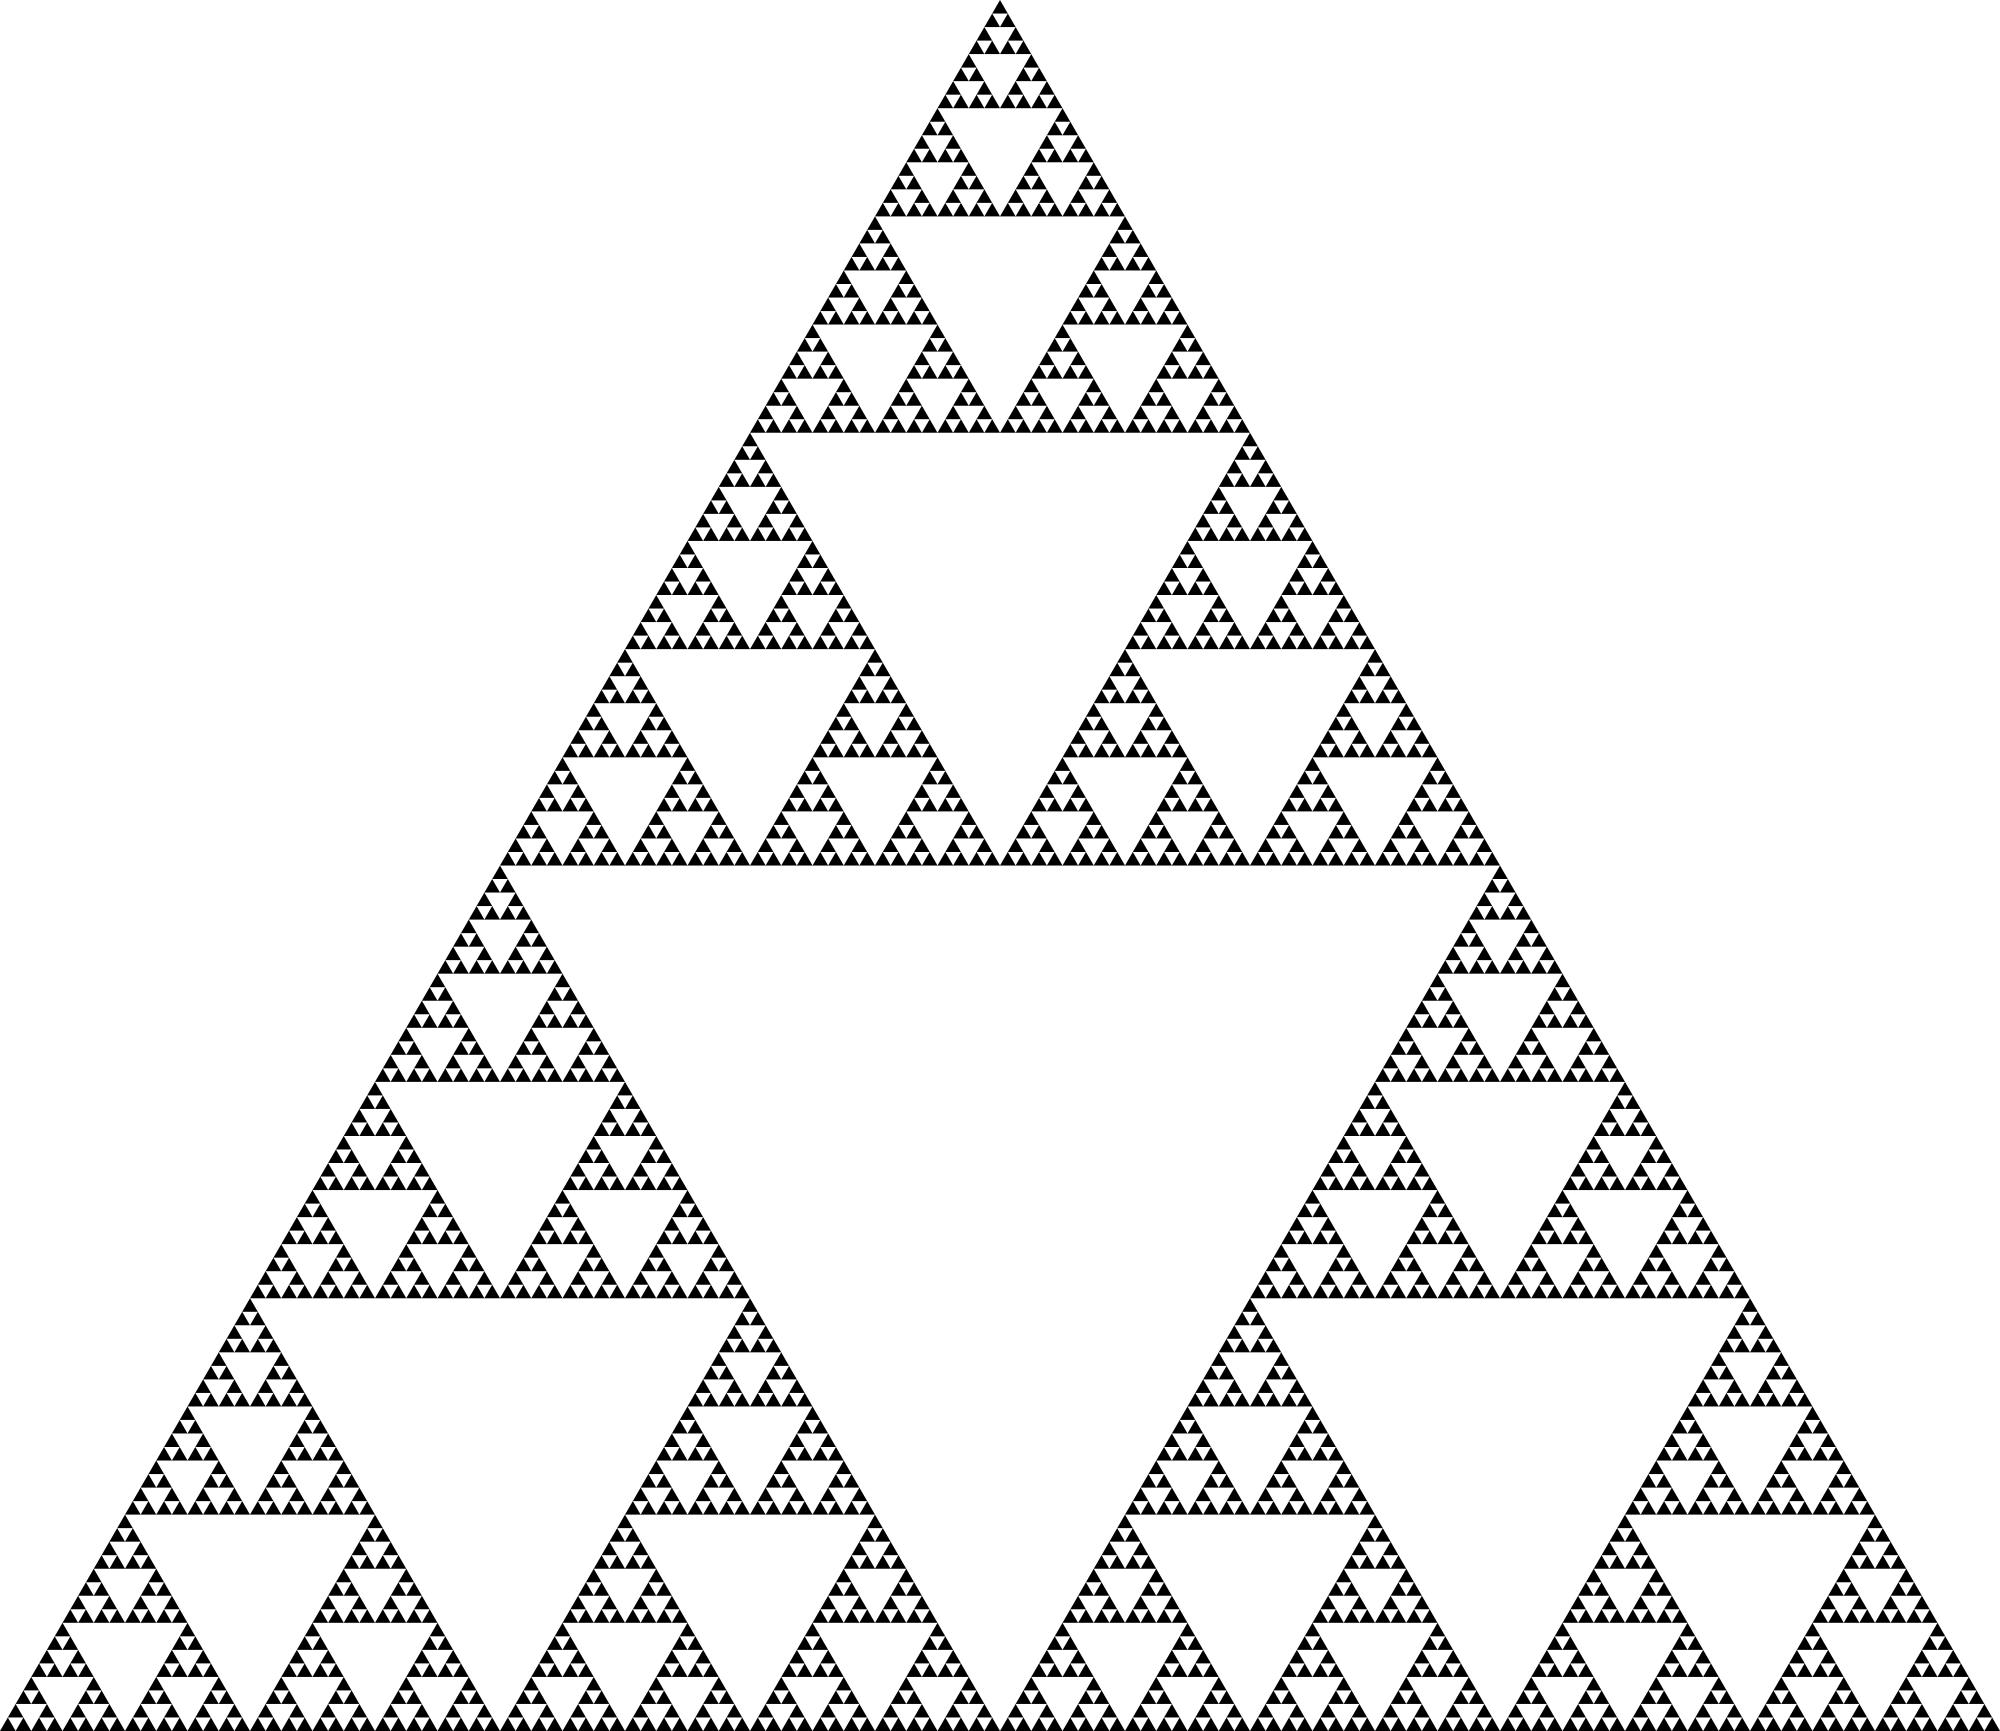
\includegraphics{hegel_by_sierpinski}}\\
Георг Гегель. Портрет математика-сюрреалиста Вацлава Серпинского.
\end{center}

\section{Наука логики Георга Гегеля}
В общем-то, см. выше. Как первый том энциклопедии, только подробнее.

\section{Философия природы Георга Гегеля}
Второй том "Энциклопедии". $\rightarrow$ механика, физика (+химия), органика. Каждая опять делится на три.

\section{Философия духа Георга Гегеля}
Третий том "Энциклопедии". $\rightarrow$ субъективный дух, объективный дух, абсолютный дух.
Субъективный дух $\rightarrow$  антропология, феноменология духа, психология. Объективный дух  $\rightarrow$ право,мораль, нравственность. Нравственность $\rightarrow$ семья, гражданское общество, государство. Государство $\rightarrow$ внутреннее право, внешнее право, всемирная история. Абсолютный дух $\rightarrow$ искусство (образная форма познания), религия (в счет идут только имеющие священное писание) и философия. Тут абсолютный дух наконец полностью осознает себя.

\section{Противоречие между методом и системой в философии Георга Гегеля}
А раз так, то вопреки \textbf{диалектике} все должно остановиться. Все, абсолютный дух все познал. Это у Гегеля, конечно, упущение. \textit{Надо было брать за основу диалектику мира}.

\section{Великая Французская революция и крах волюнтаризма.  Философия истории Георга Гегеля. }
Итак, \textbf{волюнтаризм} начал посасывть. В истории нащупывались объективные закономерности, которые свести к действиям великих людей не получалось. Например, Великая Французская Революция. Ну не могло ее не быть. Не пошел бы народ 89-м, так в 90-м бы поднялся. И вот тут-то Гегель со своим Абсолютным д-хом и выходит на сцену. История - процесс объективный. Он тоже обусловлен Абсолютным д-хом. Д-х сначала зашел в Африку и на Ближний Восток - появились Египет и Вавилон; потом пожаловал в Китай, Персию; полетал в Греции, свалил в Рим, и вот теперь обустроился в Европе. План предопределен - люди начинают осознавать замысел д-ха и претворяют его в жизнь, ибо иначе нельзя. Это сформулировано в "Философии всемирной истории" - она опубликована уже посмертно. \textit{А еще надо сказать про Гегеля и революцию. Ему принадлежит фраза "Что разумно - действительно, а что действительно - разумно". Переводя с гегельянского: разумное - нужное Абсолютному д-ху, т.е. необходимое. Т.е. бессмысленно бороться против необходимого. Оправдание стабильности а-ля Киселев-ТВ. Многим так казалось. Но Гегель же \textbf{диалектик}: то, что вчера было разумным, сегодня стало неразумным, а посему ему в действительности не место. Герцен это дело назвал "Алгеброй революции". Мораль сей басни: режим тупит - свергай его смело. Ай, товарищ майор, я не это имел в виду, только не на бутылку!..}

\section{Раскол в школе Г. Гегеля. Младогегельянцы (Давид Штраус, Бруно Бауэр).}
А  том временем Фридрих Вильгельм III сменился IV. Поменялся только порядковый номер короля. Возник кружок "Молодая Германия". В нем сидели любители Гегеля. \textbf{Правые гегельянцы} ака \textbf{старогегельянцы}, топили за консерватизм. \textbf{Левые гегельянцы} ака \textbf{младогегельянцы} же топили за реформы, а некоторые - вообще за r-r-rеволюцию. Да и против христианства (\textit{Идеалисты-атеисты. Соси, Беркли. Ах да, идеализм $\neq$ религия, если кто еще не понял}).

\underline{Давид Штраус (1808 - 1874)}. Написал "Жизнь Иисуса" (1835). В Новом Завете - 4 Евангелия. Три из них совпадают, а то, которое от Иоанна - отличается. Штраус после анализа вынес вердикт: Евангелия - мифы, хотя Христа не отрицал - ну да, был такой человек, просто про него насочиняли потом. Правда, христианином все же был.

\underline{Бруно Бауэр (1809 - 1882)}. Сначала критиковал Штрауса, потом написал "Критику священной истории синоптиков и Иоанна" (\textit{то бишь, Евангелий}). Получилось, что Христос - просто миф: почему-то его целый век не упоминают нигде, и только потом - Евангелия.

Опровергать Гегеля тоже пытались. В 1842 г. вышла книга "Глас страшного суда над Гегелем" - объявили его революционером - антихристом.
 
\section{Антропологический материализм Людвига Фейербаха}
\underline{Людвиг Фейербах (1804 - 1872)}. Родился в Баварии. Пошел в Гейдельбергский университет. Там познакомился с Гегелем и отправился в Берлин слушать его лекции. В 1828 г. перебрался в Эрлангенский университет и там читал лекции. В 1832 году написал "Мысли о смерти и бессмертии". Веруны раскукарекались и выперли из университета с волчьим билетом за безбожие. \textit{С волчьим. Сволочи}. С 1836 г. поселился в деревне, в в 1839 г. написал "Критику философии Гегеля". Стал \textbf{материалистом}. В 1841 году пишет свою главную работу - "Сущность христианства", в которой и расписывает свою философию. 

Материализм свой назвал \textbf{антропологическим}. В центре - человек. Нет духа, кроме человеческого духа, да и тот - продукт мозга. Итак, природа первично, а сознание - продукт природы. Материя существует в пространстве, которое тоже объективно. Материя движется; более того, движение есть способ существования материи. Да, движение есть не только механическое. В мире нет ничего непознаваемого, но есть непознанное. Мышление же раскрывает сущность вещей. Чувства же дают ему материал.

В той же работе, он пишет про историю религии (собственно, именно ей и посвящения книга, если смотреть по заглавию). Религия - не просто фантазия от незнания, а отражение реального мира - хоть и адски искаженное. А с обществом Фейербах опять скатывался в идеализм, хоть и искал природный корни морали и т.д. Да, в атеисты Фейербах подался еще до того, как стал материалистом. \textit{Да, нельзя мешать идеализм и религию, сколько можно повторять! Семенов за это на пересдачу отправляет - по глазам видно.} 

\section{Исторические предпосылки возникновение марксизма. Основные части марксизма.}
Итак, в Западной Европе сформировался \textbf{капитализм}. И рабочему классу жилось очень плохо. Рабочий день доходил до 16 часов (\textit{В сессию бывает и хуже. В прочем, это не у станка стоять.}). Да, для детей от 8 до 12 лет рабочий день ограничили до 12 часов. 8 часов в день - завоевания Октября (\textit{хотя встречал я инфу, что где-то и до Октября установили 8-часовой рабочий день. Впрочем, возможно это было на отдельных фабриках}). Социалочка тоже отсутствовала. О рабе хотя бы заботились более-менее - если заболеет и сдохнет, будет печаль. А тут можно нанять нового! Тоже за копейки, ибо иначе он с голоду умрет. Ну и естественно, в рабочих проснулась ненависть. Нет, не так. \textbf{НЕНАВИСТЬ БЛДЖАД!!!!}.
Например, были \textbf{луддиты}, громившие машины (название произошло от Неда Лудда, возможно, мифического аки Иисус). Естественно, капиталистам это не понравилось. Парламент (а заседают в нем ни фига не рабочие) ввел закон - вешать. Во Франции, в Лионе восстали ткачи - войска справились только с подкреплением. А потом и Силезские ткачи восстали. В Англии появилось \textbf{чартистское движение}. Оно типа за рабочих, только вот незадача - избирателей в Англии $1.5 \%$. Провели реформу - и народ зажил (\textit{нет}): $4.5 \%$. Да и то сплошные буржуи. Место в парламенте можно было даже купить. Чартисты потребовали всеобщего избирательного права (\textit{впрочем, только для мужчин - вы пока в пролете, дорогие феминистки}). В 1840 году появилась первая партия рабочего класса - \textbf{Национальная Ассоциация Чартистов}. Утописты же начали рисовать картины светлого будущего, в котором не будет частной собственности. \textit{Итак, лирическое отступление номер-$\aleph$. \textbf{Частная собственность} - это собственность, с помощью которой один класс эксплуатирует другой, живя за его счет. \textbf{Личная же собственность} - это собственность, владельцем которой является один человек. В веке капитализма кажется, что это одно и то же, но нет: личная собственность не всегда частная, а частная - не всегда личная. Пример личной, но не частной собственности - скажем, зубная щетка: у нее один владелец, но никто не вынужден отдавать часть продукта труда из-за того, что зубная щетка не его, а капиталиста. Пример частной, но не личной собственности - Древний Египет. Быдло впахивает на полях, которые принадлежат знати. Причем не каждый кусочек принадлежит кому-то одному, а все всем. То есть да, взять и загадить кусок плодородной почвы, потому что он твой, нельзя. Другой пример  - ВНЕЗАПНО - СССР. Да-да, это называлось "Социализм в отдельно взятой стране${}^\mathtt{TM}$", но на деле были рабочие и номенклатура, и с их расслоением по доходам, а еще со спецполиклиниками/служебными квартирами/спецмагазинами об отсутствии эксплуатации можно было говорить, только бессовестно перевирая Маркса/Энгельса, впихивая цитатки к месту и не к месту. Рассказывают, что Сталин оставил после себя только шинель и пару сапог (а, ну и атомную бомбу в стране, которую принял с сохой) - на всем остальном были инвентарные номера. Так вот, бирки с цифрами вовсе не мешали членам${}^\mathtt{TM}$ пользоваться роскошью. Да, жировали. Да, при Кобе в том числе. Убери ледоруб, дорогой сталинист. Это все к чему. Если какой-нибудь директор вдруг решил бы развалить свой завод, при капитализме всем было бы плевать. В СССР же это - срок, а то и расстрел за уничтожение "народной" собственности в особо крупном размере и циничной форме. Так что собственность частная, но не личная. И последнее. Ту же зубную щетку можно представить и как частную собственность (тут вдруг война, нет швабр, полы драят щеткой), и как коллективную (в данном случае лучше не представлять). Это показывает, что частная и личная собственность есть характеристика отношений, а не отдельно взятой вещи. Поэтому Энгельс с Каутским спорили не зря, а Шариков со своим "отнять и поделить" сосет болт. Dixi. 
}
Да, уже никто не помнит, что было до отступления. А были там утопические социалисты - например, А. Сен-Симон, Р. Оуэн, Ш. Фурье, которые мечтали о светлом коммунистическом будущем. Огромные дома - коммуны, все регламентировано - прямо Сталингулаг какой-то. Предлагали строить коммуны и так постепенно все заполнить. Даже думали, прогрессивная буржуазия поддержит планы по лишению ее рабочих рук. Разумеется, нужен был нормальный план. А для этого нужно описывать общество и историю. А для этого нужна их объективная основа. Ответ такой : социальная материя - это \textbf{экономика}, система производственных отношений. Значит, в теории необходима политэкономия. Ну а потом - нечего ждать милости от капиталистов, товарищ, берем и устраиваем r-r-rеволюцию${}^\mathtt{TM}$. После переходного периода распределение будет по труду, а потом производительность труда повысится настолько, что и просто по потребностям. Эксплуатация человека человеком будет уничтожена (\textit{к роботам это не относится - они как раз и будут впахивать}). 

\section{К. Маркс и Ф. Энгельс как создатели марксизма. Эволюция их взглядов.}
\underline{Карл Маркс (1818 - 1883)} - Трир, Рейнская республика, Пруссия. Родился в семье адвоката, перекрестившегося еврея. Окончил гимназию, перешел сначала в Боннский, а потом и в Берлинский университет. Стал младогегельянцем. В 1841 году защитил докторскую диссертацию (\textit{магистерский диплом в нашем понимании}). Был редактором "Рейнской газеты", республиканцем и любителем революции. В том же году (1843) газету закрыли. Маркс переехал во Францию, и там в 1844 году подружился с Энгельсом.
 
\underline{Фридрих Энгельс (1820 - 1895)} Родился в Бармене, в семье капиталиста (\textit{любил ломать стереотипы}). Учился в гимназии, но не окончил из-за отца, которому нужен был наследник - управленец. В 1841 пошел в армию вольноопределяющимся. Служил в Берлине, встретился с Бауэром и стал младогегельянцем. Отец послал в Англию. Энгельс там изучает рабочий класс. В 1845 году пишет "Положение рабочего класса в Англии". Еще до знакомства изучил Фейербаха и подружился с Марксом. 

Решили запилить новый материализм. Пишут "Наброски критики политэкономии" - там пишут, что экономика - основа. "Святое семейство" - критикуют младогегельянство. В "Немецкой идеологии" запиливают материалистическое понимание истории (1845), правда пока что в общих чертах. Опубликовали же ее только в СССР. Вступили в "Союз справедливых", потом он переименовался в "Союз коммунистов". Пишут "Манифест коммунистической партии". Маркс возвращается в Германию, и в свежезапиленной им "Новой Рейнской газете" призывает к революции (пока что буржуазной). Энгельс же поучаствовал в вооруженном восстании, и был приговорен к казни. Сбежал. Марксовскую же газету закрыли, а самого чуть не посадили. В 1864  году образован 1-й Интернационал. Рабочие начинают бороться, и капитализм сдает. Создаются фабзавинспекции. А Маркс тем временем пишет "Капитал". Первый том был сдан в печать в 1867 году. Маркс говорил, что рано, но Энгельс настоял. Еще два тома дописаны так и не были. Энгельсу пришлось уже после смерти Маркса дорабатывать.

\section{Философская и обществоведческая мысль в поисках объективного общественного бытия и движущих сил истории}
Итак, Гегель создал философию истории - объективного процесса. Но там есть "черный ящик" - тот самых Абсолютный дух. Нужно же что-то более определенное.  Где искать объективные начала общества? Не ясно. Да и с историей все так же: или великие люди, или Абсолютный Д-х какой-то. Как же построить нормальную общественно-историческую философскую теорию? Для этого нужно было найти социальную материю. Первый шаг сделали французские историки эпохи Реставрации.

\section{Французские историки эпохи Реставрации}
 Итак, французские историки эпохи Реставрации: \underline{Огюстен Тьерри}, \underline{Франсуа Гизо}, \underline{Франсуа Минье}, \underline{Адольф Тьер}. Они открыли \textbf{классы} и \textbf{ классовую борьбу}. Были догадки и до этого, но они разработали теорию. \textit{Да, эпоха Реставрации - это когда вернулась монархия в лице Людовика XVIII-го. Буржуазию оттеснили, но монархия конституционная. Потребовалось обоснование того, что буржуазии нужна власть.} Так вот, идет борьба за власть для защиты объективных интересов. Были феодалы и крестьяне - крестьяне вынуждены кормить феодалов, потому что земля ихняя. \textbf{Классы} - большие группы людей, занимающих разное положение в системе имущественных отношений. Фундаментальное отношение - собственность. Да, а великие люди только лучше других понимали интересы своего класса. Уклад сменяется другим, а имущественные отношения те же - непорядок. Гизо в "Английской революции" объяснял феодализм завоеваниями. Пришли, и сказали, что теперь тут их земля.


\section{Философская и обществоведческая мысль в поисках объективного источника общественных идей. Открытие экономических отношений и возникновение политический экономии.}
Про капитализм писали меньше. Однако, нашлись и такие. \underline{Реналь} и \underline{Ленге} поняли, что и буржуазия с рабочим классом находятся в состоянии классовой борьбы. Тут надо сказать, что \textbf{экономические отношение собственности} - распределение и обмен - прикрыты \textbf{правовыми} и не заметны. При капитализме на первом плане обрабатывающая промышленность. Нужна координация - и тут рыночек решает и без рабства/феодалов. Более того, они мешаются. Производство же происходит ради прибыли. Но рабочие вынуждены продавать свою силу, пусть и по экономическим причинам (с голоду сдохнут иначе). Естественно встал вопрос, как же поднимать экономику и обустроить \%countryname\%. Первыми тут отличились \textbf{меркантилисты}. Богатство - это золото и серебро, значит, их нужно ввозить, и поменьше вывозить. \underline{А. Монкретьен} в 1615 году написал "Трактат о политической экономии". Встала проблема цены и стоимости (\textit{это разные вещи: цена - это то, сколько просят на рынке, стоимость же есть объективное свойство вещи, делающее ее сравнимой  другими}). Ее решила "Классическая буржуазная экономия" \underline{У. Петти}. Потом подтянулись \underline{Адам Смит (1723-1790)} с его "Исследованием о природе и причинах богатства народов" (1776) и "невидимой рукой рынка", и \underline{Давид Рикардо (1772-1823)} с его тремя типами доходов: \textbf{рентой},\textbf{прибылью} и \textbf{заработанной платой}. \textit{Позднее Маркс скажет, что первые две - одно и то же}.

\section{Философская и обществоведческая мысль в поисках объективного источника общественных идей. Выделение основных эпох истории цивилизованного общества.}
Итак, при капитализме нашлись экономические отношения. Откуда они? Ну есть и все. Человек уж так устроен - такая у него природа. История же подошла с другой стороны. Мы помним вопрос про периодизации. Однако же была еще периодизация цивилизованного общества: \textbf{античность}, \textbf{темное время} ака \textbf{Средневековье} и \textbf{Возрождение} [античной культуры] ака Новое время. Она родилась из очевидно различной культуры этих эпох. В 17-м веке такую периодизацию поддерживал Кристоф Келлер. Он даже написал по книге на каждый из этих трех периодов. \textit{Так и сейчас периодизируют, только добавили \textbf{Новейшее время}}.

Стали исследовать античный мир. И тут выяснилось, что там процветало \textbf{рабство}. А в Средневековье - крепостные. Они уже не рабы, хоть и феодально-зависимые. А при капитализме в Новом времени- зависимые экономически рабочие. А потом до кучи еще открыли Восток. 
\underline{Франсуа Бернье (1620-1688)} Попутешествовал по Востоку, написал "Историю политических потрясений в государстве Древнего Могола" Удивительное дело - порядки одни на весь Восток, но не те, что знала Европа. А потом Англия завоевала Индию. Ее стали изучать. Так и появилась теория с четырьмя эпохами. Это уже и Гегель учитывал.

\section{Философия истории А. Сен-Симона}
\underline{Анри Сен-Симон (1760-1825)}. Уже встречался ранее как \textbf{утопический социалист}. Выделял три эпохи - античность, средневековье, Новое время. Каждая определялась общественными порядками. А дальше - утопический социализм. Но остался вопрос - почему рабство/крепостничество/наемный труд сменяли друг друга? Сен-Симон говорил по общечеловеческий разум. Он порождает порядок, перерастает его, создает новый. И т.д... \textit{Надо сказать, такой концепции придерживаются до сих пор. Фукуяма, например. Только у него все же наступил конец истории в виде сегодняшней либеральной демократии и капиталистической экономики (второе подразумевается необходимым условием первого)}.

\section{Экономический детерминизм Ричарда Джонса}
\underline{Ричард Джонс (1790-1853)}. Окончательно сформировалась политэкономия. Определил ее как науку о формах производства и распределения материальных благ. И экономические отношения главенствуют. Создатель концепции "Экономического детерминизма" - фундамент истории - экономические отношения. Капитализм у  него тоже не вечен, \textit{хотя назвать Джонса социалистом никак нельзя - он консерватор}. 

\section{Создание материалистического понимания истории и его основные понятия}
Итак, на вопрос "Почему же порядки сменяют друг друга" ответа так и не было. И вот тут наконец появляются \underline{Карл Маркс} и \underline{Фридрих Энгельс}. Они исследовали общие закономерности развития капитализма. И понеслось... Во-первых, было сформулировано чем человек отличается от животных. Животные приспосабливаются к природе, и максимум, что они могут сделать - это муравейник. У человека же вся жизнь построена вокруг создания таких предметов, которых в природе нет и не может быть. Закончится производство - закончится история человечества. А производство - процесс общественный - ведь сообща можно достигнуть куда большего, чем в одиночку, не говоря уже про дифференциацию труда со времен охоты и собирательства (\textit{Впрочем, сами по себе они на производство не тянут. А вот копья и каменные топоры, шкуры на одежду и ожерелья, горшки и т.д.  - это оно}). Да, для упрощения процесса труда изготавливаются орудия труда. Затем, производство уперлось уже в физиологию. Стали появляться машины. Вводится понятие \textbf{способа производства} - это как раз экономические отношения, и \textbf{общественно-экономического уклада} - "общественная оболочка" способа производства. Так вот, мы подходим к следующему вопросу - тому самому идеализму в социологии. Итак, общественное сознание определяет общественную среду. Но бытие определяет сознание. Итак, порочный круг разорвался: уровень производительных сил - \textbf{базис} - определяет сознание, которое уже творит \textbf{надстройку} - общественно-экономические отношения. Таким образом, историческое развитие - естественный процесс : развивается базис, надстройка отстает, сознание ее перестраивает - отсюда и революции. Всего были четыре эпохи - азиатский способ, рабство, феодализм, капитализм. Дальше, как известно, предсказывали \textbf{коммунизм}  - но это уже футурология, а не история. Надо сказать, что азиатский способ производства изучили только в 20 веке. \textit{И кстати, в СССР  дважды разгоралась дискуссия, и оба раза ее прекращали сверху. В первый раз - еще при Сталине и с расстрелами в том числе. Второй раз Семенов уже застал лично. Надо сказать, он сам исследовал этот способ производства. Говорит, работу приняли только через 10 лет да и то чудом. А все, возможно, потому, что азиатский способ производства, как уже писалось ранее, слишком смахивал на советские реалии}.

\section{Возникновение диалектического материализма и его отличие от всех предшествующих материалистических систем}
Перед материалистами стояла еще одна проблема: сознание постоянно было пассивным, потому что иначе оно бы определяло бытие, и был бы идеализм. \textit{Тут, вероятно, следует сделать последнее лирическое отступление. Оно на правах гипотезы автора, и ни в коей мере не претендует на истину в последней инстанции. Дело в том, что философия - не только онтология, но и общий метод исследования, в том числе метод исследования самого себя. Так вот, казалось бы, что плохого в том, что сознание может влиять на материю, если сознание - просто продукт куска материи? Вроде бы, мы от материи не отказываемся - просто сложное взаимодействие  в системе из очень сложно сгруппированных атомов. Однако, если дальше, приняв эту мысль, попытаться объяснить что - либо, мы неизбежно начнем сваливаться к мысли о первичности сознания, и все наши рассуждения приобретут идеалистический окрас, со всеми вытекающими проблемами идеализма (например, черный ящик Абсолютного духа или берклиевский солипсизм). Для сравнения - идеалист, вероятно, придет к выводу о том, что красота есть нечто первичное и априорное, вульгарный материалист, особенно атомист и механистический редукционист, скажет, что эти понятия сформировались окружающей средой, но не более того - ведь все движение он пытается без остатка свести к механическому, игнорируя закономерности более сложных структур, или пытаясь вывести их из механического движения атомов. Последовательный же материалист... Почитайте "Лезвие бритвы" Ефремова, сцену, где главгерой Гирин рассуждает о природе красоты с позиций диалектического материализма. Это действительно последовательное и логичное рассуждение, способное делать предсказания, даже если Ефремов в лице главгероя и не прав в каждом из тезисов (например, у биологов может подгореть с некоторых опытов Гирина). Вкратце - понятие красоты сформировалось из понятия целесообразности/здоровья/пригодности в пищу еще когда человек даже не прямоходящий был}. Так вот, Маркс с Энгельсом наконец смогли сделать сознание активным - оно отражает мир, но способно действовать. Самое характерное же в том, что они предсказали, что даже само сознание сформировалось после того, как человек (обезьяна) начал что-то делать. Палеонтологи потом подтвердили - труд сделал из обезьяны человека. Действительно, что-то и как-то сделать может и животное. Но это все держится в том числе на инстинктах. Для того же, чтобы понимать, что делать и как, нужно прокачать межушной нервный узел. Что в ходе эволюции и сделали обезьяны где-то так 2 млн лет назад. Маркс и Энгельс создали \textbf{диамат} ака \textbf{диалектический материализм} - как бы Гегель, только перевернутый с идеалистической головы на материалистические ноги. Сделан он был на основе \textbf{материалистического понимания истории} ака \textbf{исторического материализма} ака \textbf{истмата}. Кроме этой проблемы, он решил еще и проблему общего и отдельного, объяснил, как общее проникает в нашу голову из мира, и наконец, решил проблему свободы и необходимости.

\section{Классическая и неклассическая западноевропейская философии Нового времени. Их отличие и особенности их развития.}
Все, что было рассмотрено выше - это классическая философия. А была еще и неклассическая. И что-то про них Семенов не говорил. Впрочем, ничего. В неклассической философии поднимались другие темы, то есть это уже не та философия-наука-об-истине-и-методе-мышления.
\end{document}
